
\section{Selecting Platforms in CLIC}

A logical plan needs to be transformed into a physical plan before being actually executed.
That is, selecting each logical operator a physical platform to transform to the physical operator.
However, assuming that a logical plan has N operators, and each operator has K available physical platforms to choose from, 
there exist $K^N$ available combinations.
Even so, there is still a best platform for each operator, on which deploying the operator can achieve the best overall performance. 
We take the best platform as the label of this operator.
The label of one operator is not fixed, but change by multiple factors.
Therefore, the goal of the platform selection is CLIC is to find this label for each logical operator in a logical plan to achieve the best overall performance.


In CLIC, a logical plan is organized in the form of DAG where the node denotes the logical operator and the edge denotes the operator dependency.
Selecting the label of each node in a graph is actually a typical node classification problem.
Such problems with topology as input are usually solved with the Graph Neural Network(GNN) because it can be directly applied to the graph structure without encoding it to a vector first[].
Among many GNNs, GCN is considered better at solving the node classification problem because of its ability of capturing neighbor relationships with its convolution kernel[].
Compared with the ML-based a pproach, GCN avoids the loss of structural information due to the need of encoding the topological structure as a vector[];
One more step before feeding the logical plan into GCN is to vectorize the operator, i.e transform the operator object into a numerical vector.
However, as we have disscussed in Section 2.2, the traditional vectorization method is not suitable for CLIC. 
% those drawbacks ? 第二章要不要说呢?说了的话这能直接用 the、those 吗?
Inspired by the word embedding[], we propose a novel feature extraction method called the operator embedding and overcome those drawbacks for the first time.
In 5.1, we give a first look to the the naive encoding approach and discuss its limitations, and then we introduce our novel embedding-based encoding.
In 5.2, we detailed the process of using GCN to select platforms through an example.
In 5.3, we introduce the method of synthesizing training data of the operator embedding and the GCN.

\subsection{Feature Extraction}
As it turns out, many Machine Learning algorithms and almost all Deep Learning Architectures are incapable of processing raw form data like plain text or, in this case, the operator object. 
% 简单点,说话的方式简单点
They require numbers as inputs to perform jobs like classification, regression etc. in broad terms. 
Therefore, the operator needs to be encoded as the numerical vector before fed into GCN.

When designing the feature vector, we consider the following three most influential factors: the operator itself, hardware, and workload.

\subsubsection{Operator Encoding}
Operators describe the computation logic of the workflow.
Two logical plans with the same topology can be different because the consisted operators are from two domains.
As examplified in Figure \ref{fig:graph-comparison}, although both of the two plans have the same topology,
\ref{fig:same-graph-sql} describes a SQL query while \ref{fig:same-graph-linear} is a mathmatical calculation.
As a result, they need to be classified to the different execution engines, such as Postgre for Figure \ref{fig:same-graph-sql} and Tensorflow for the other.

\begin{figure}
  \subfigure[SQL Query]{
      \label{fig:same-graph-sql}
      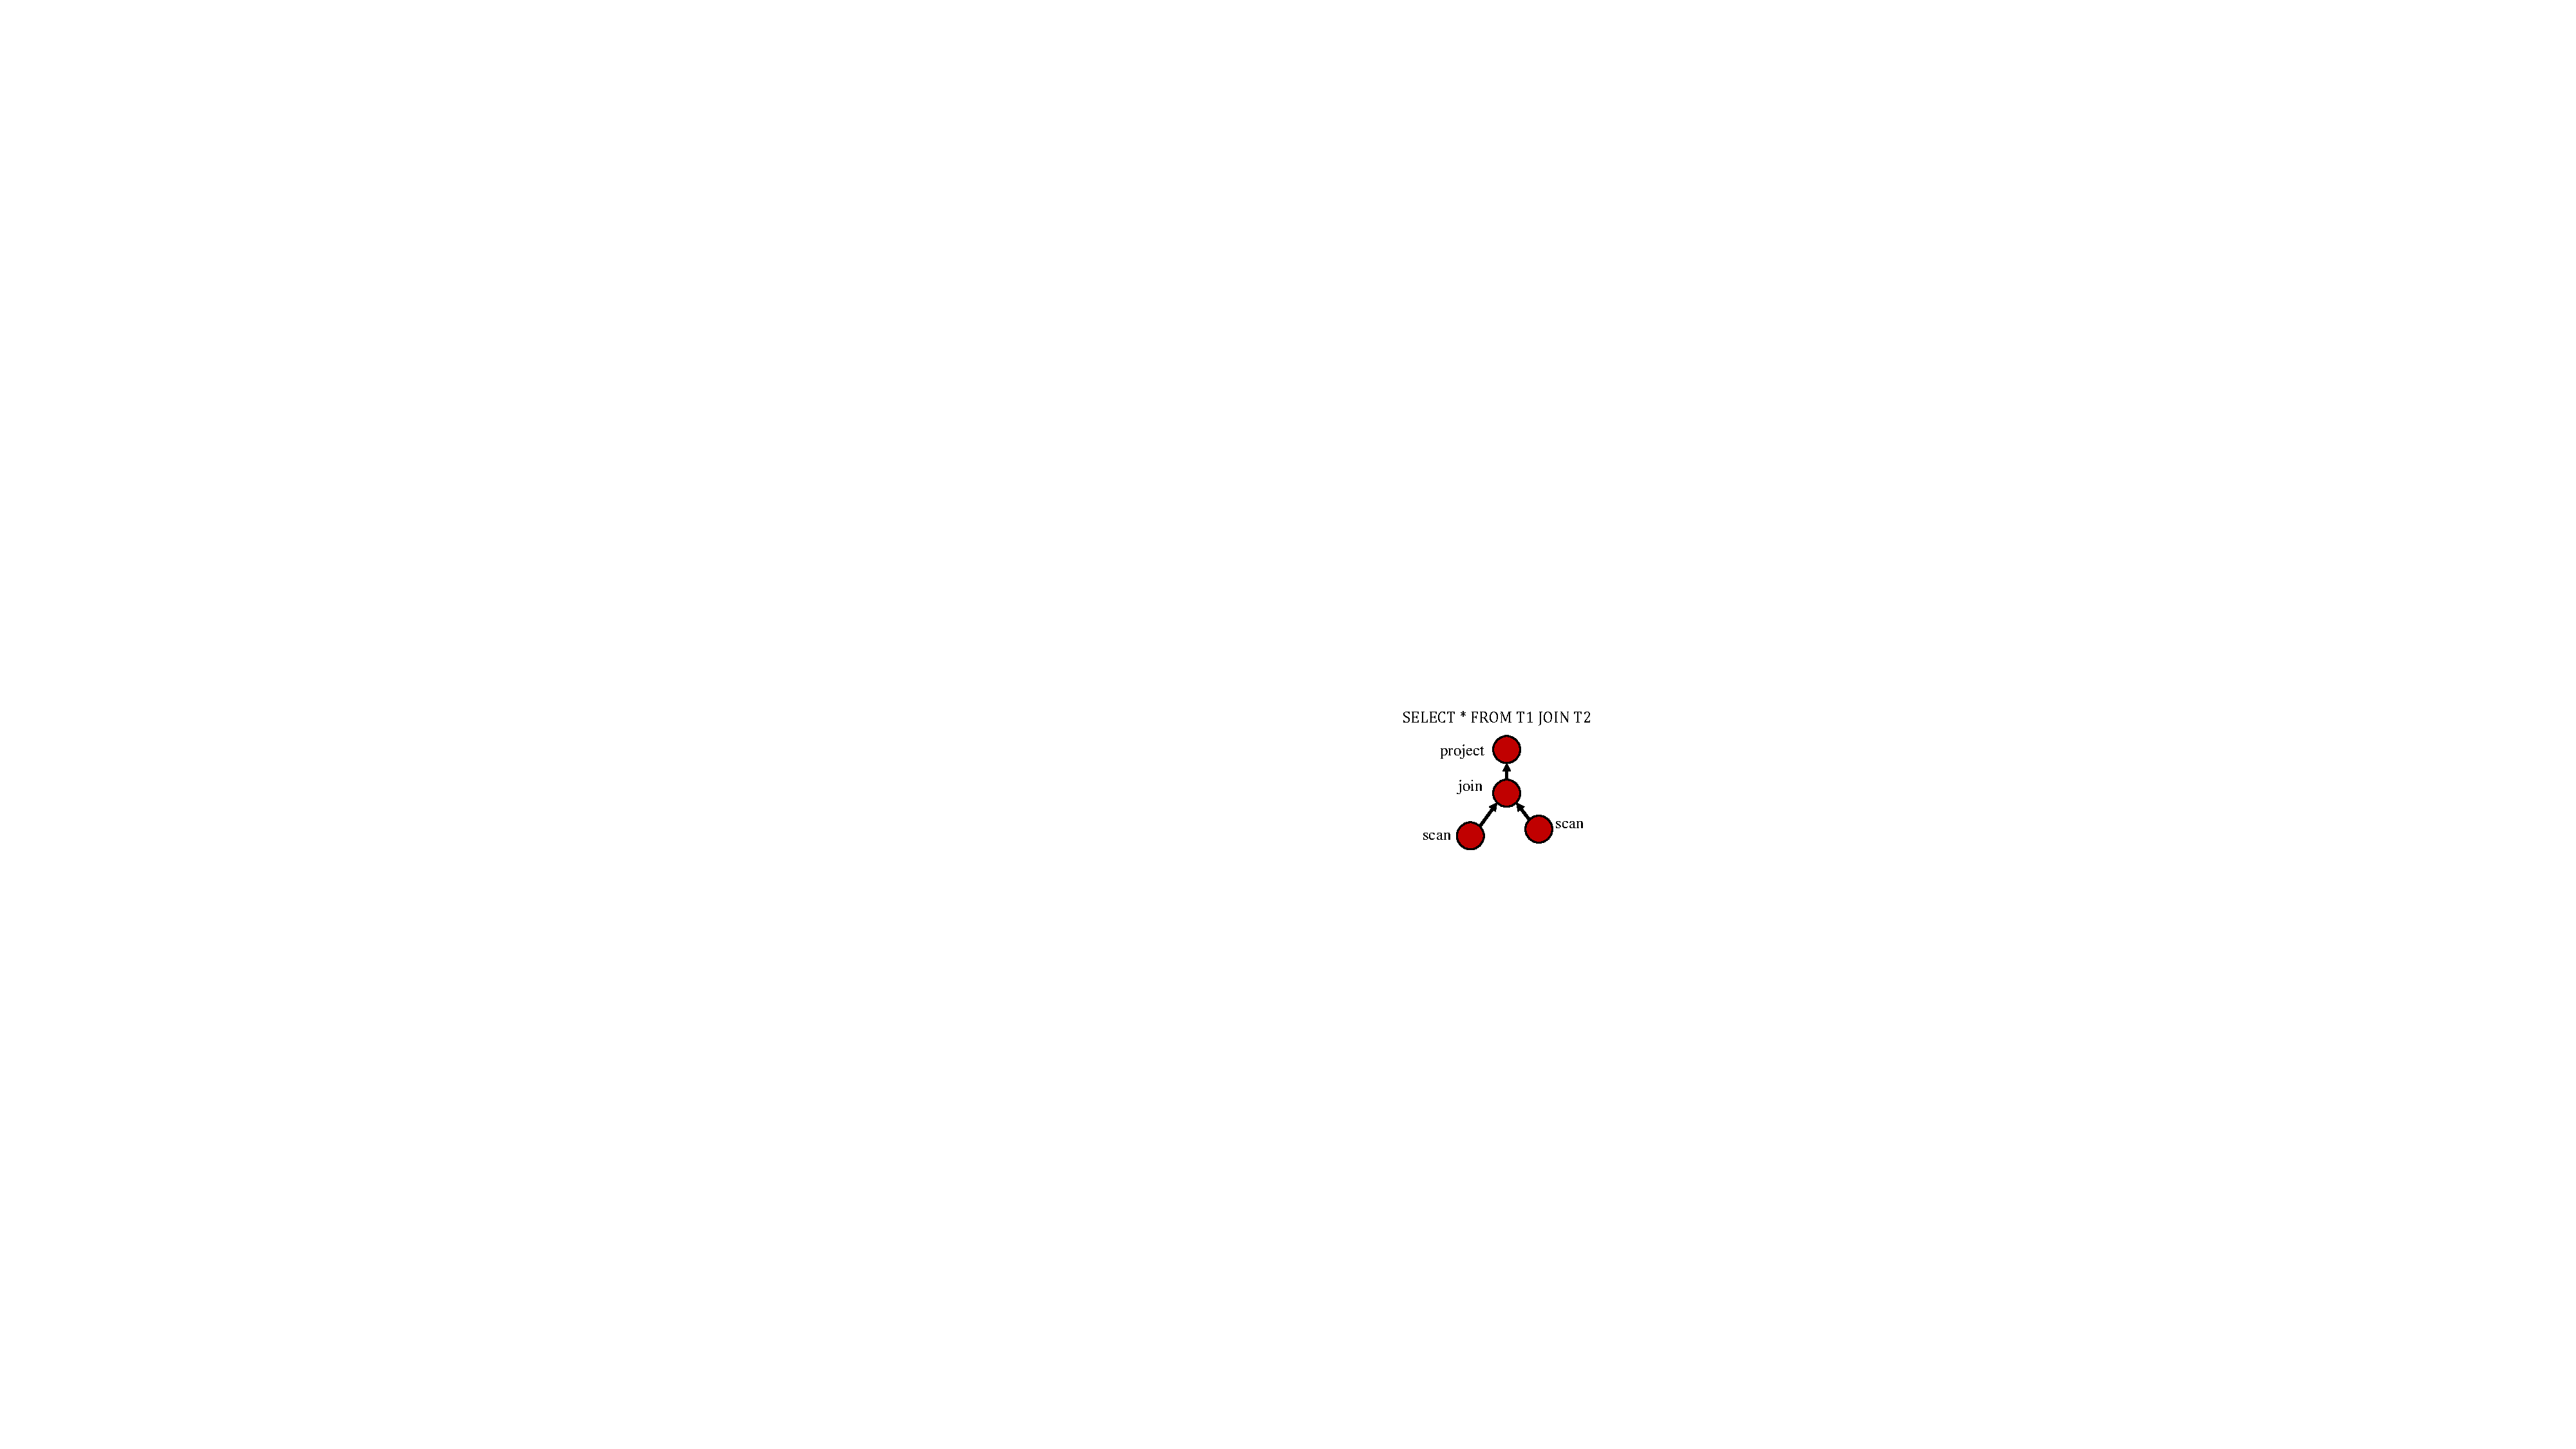
\includegraphics[width=0.36\linewidth]{figures/same-graph-sql.pdf}
  } 
  \subfigure[Linear Algebra]{
      \label{fig:same-graph-linear}
      
\includegraphics[width=0.3\linewidth]{figures/same-graph-linear.pdf}
  } 
  \caption{Plan with the same structure}
  \label{fig:graph-comparison}
\end{figure}

We first follow the traditional approach that using the one-hot encoding to represent the operators.
\textbf{One-Hot Encoding}
One-hot encoding is an simple but effective vectorization method that has been widely adopted in vectorizing the category features, such as gender or id. 
The vectorization result is a 0-1 vector whose dimension is equal to the number of categories.
The blue segment of the feature vector in Figure \ref{fig:feature-vector-onehot} illustrates the one-hot encoding. 
As we can see that, each row stands for an operator and only has one non-zero element at its corresponding column.

\begin{figure}
  \subfigure[One-Hot Encoding]{
      \label{fig:feature-vector-onehot}
      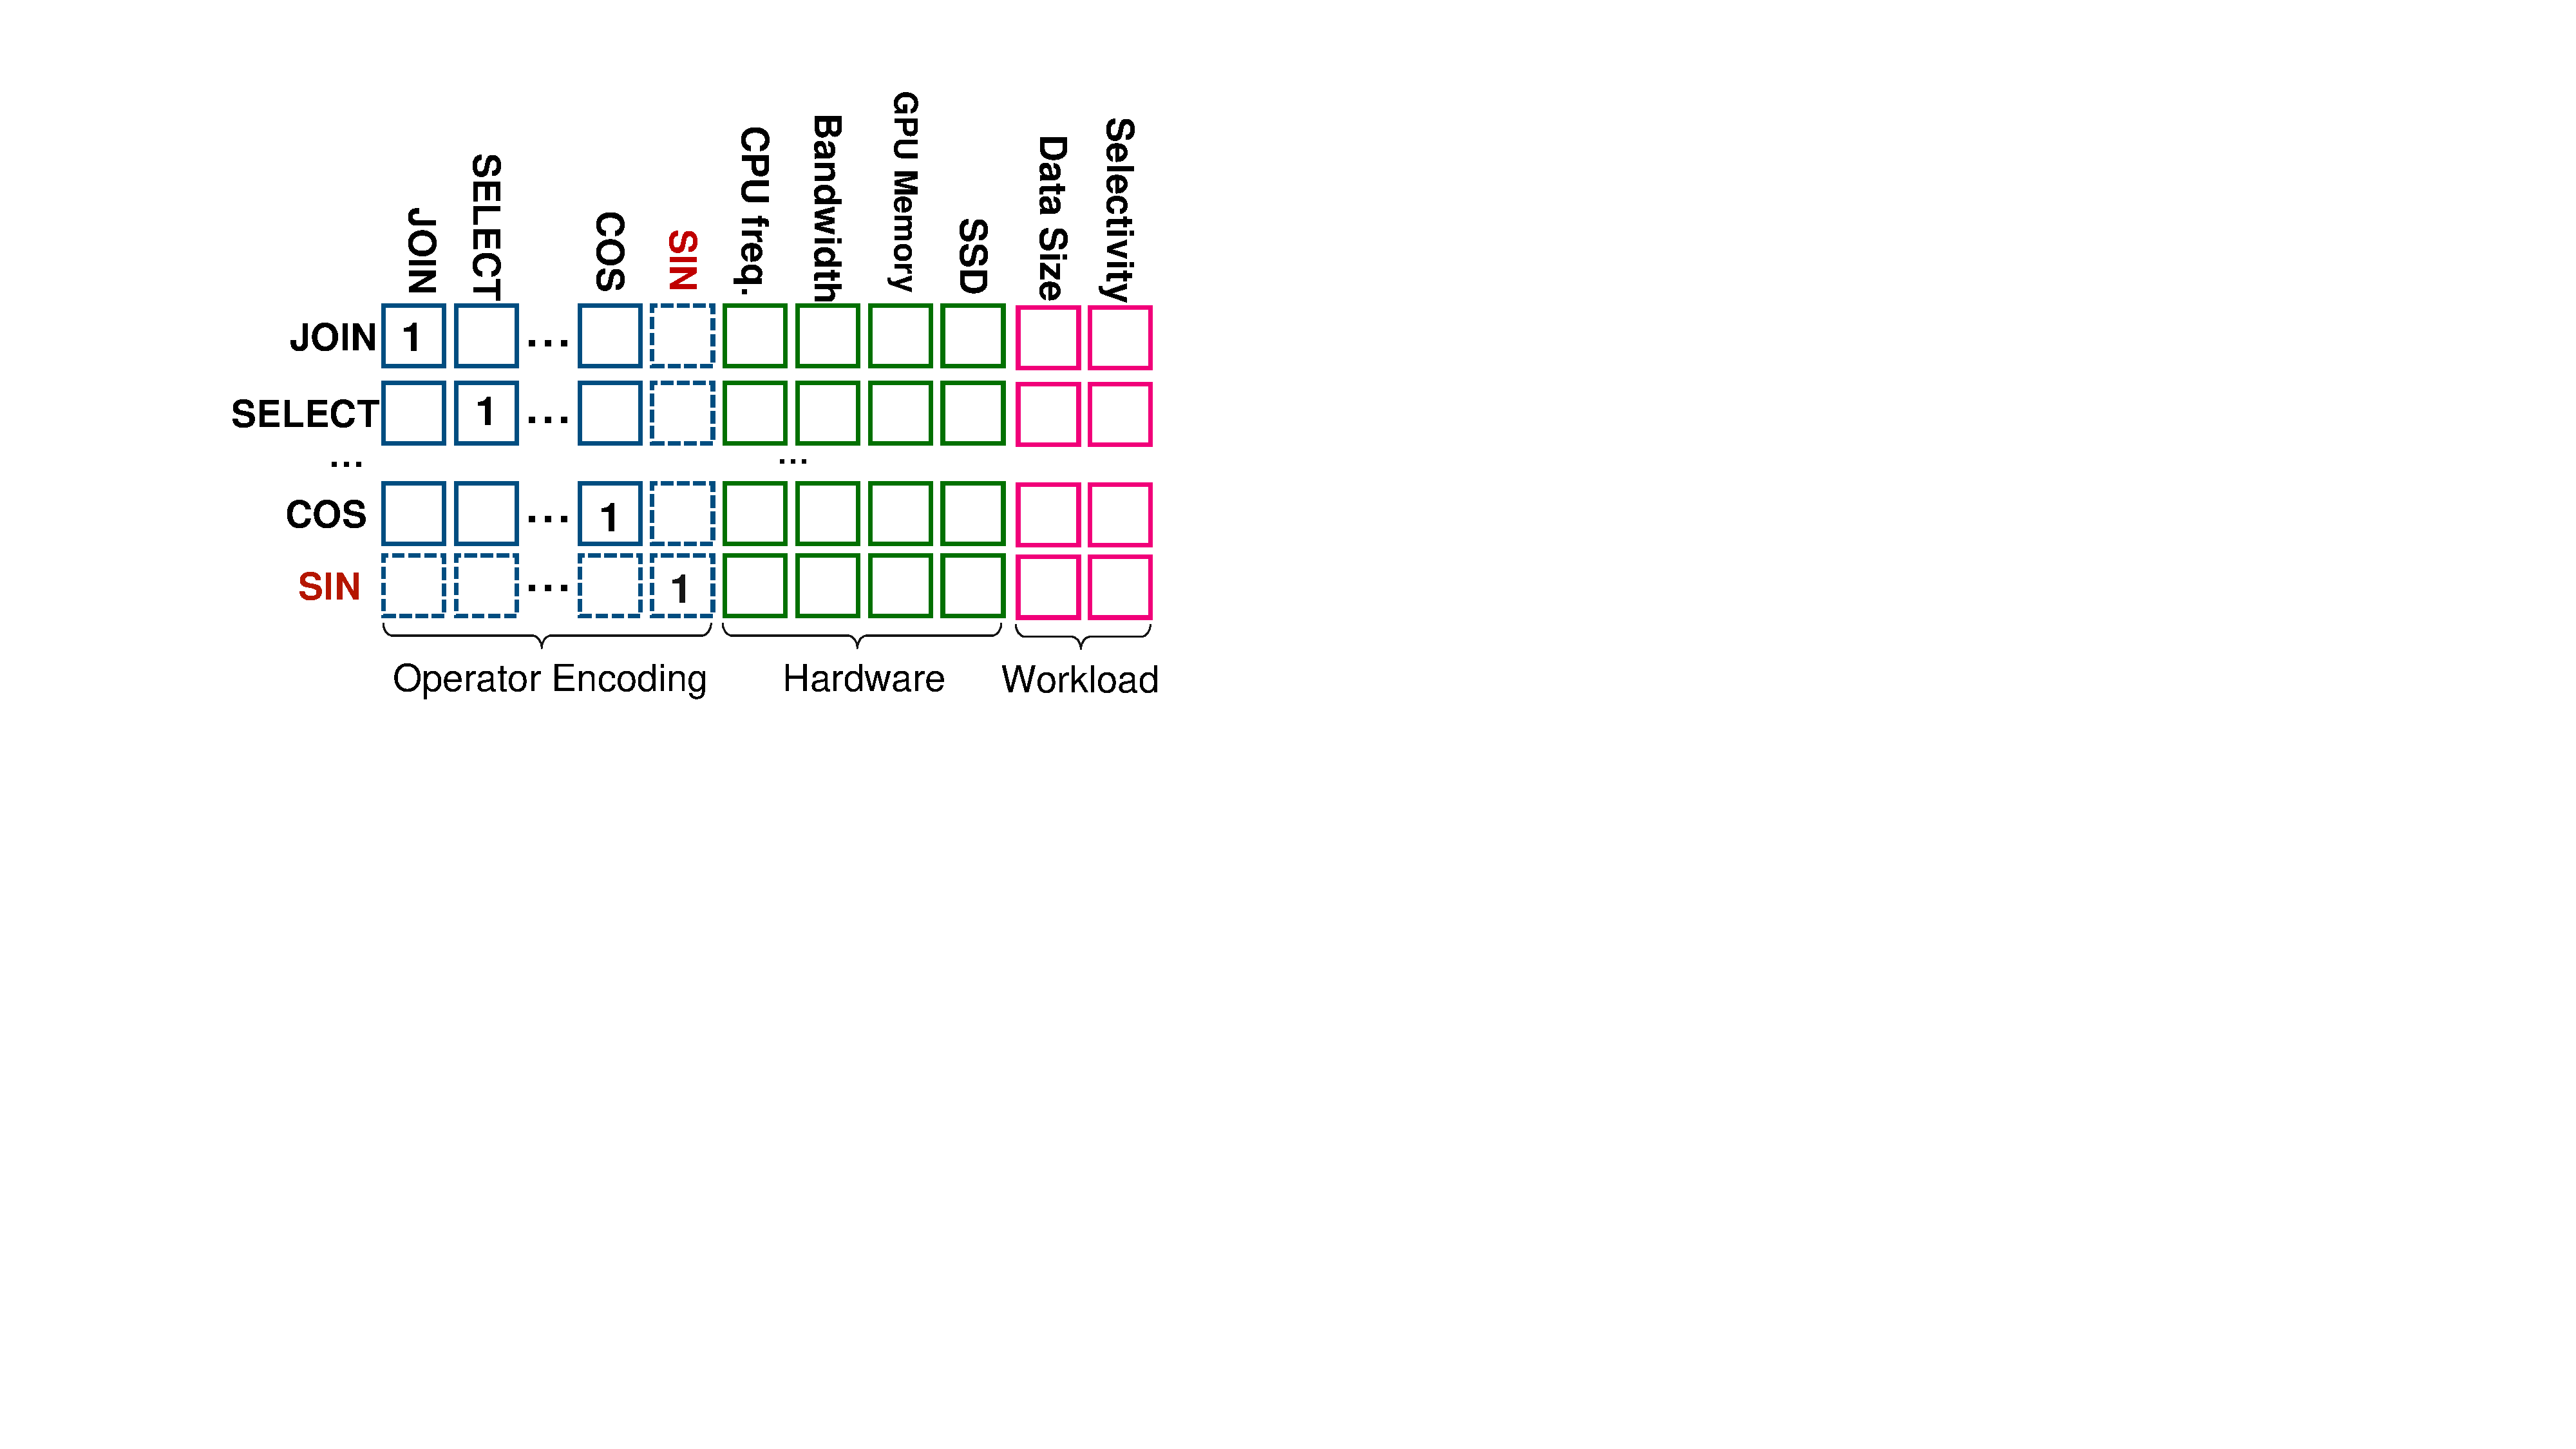
\includegraphics[width=0.45\linewidth]{figures/feature-vector-onehot.pdf}
  } 
  \subfigure[Operator Embedding]{
      \label{fig:feature-vector-embedding}
      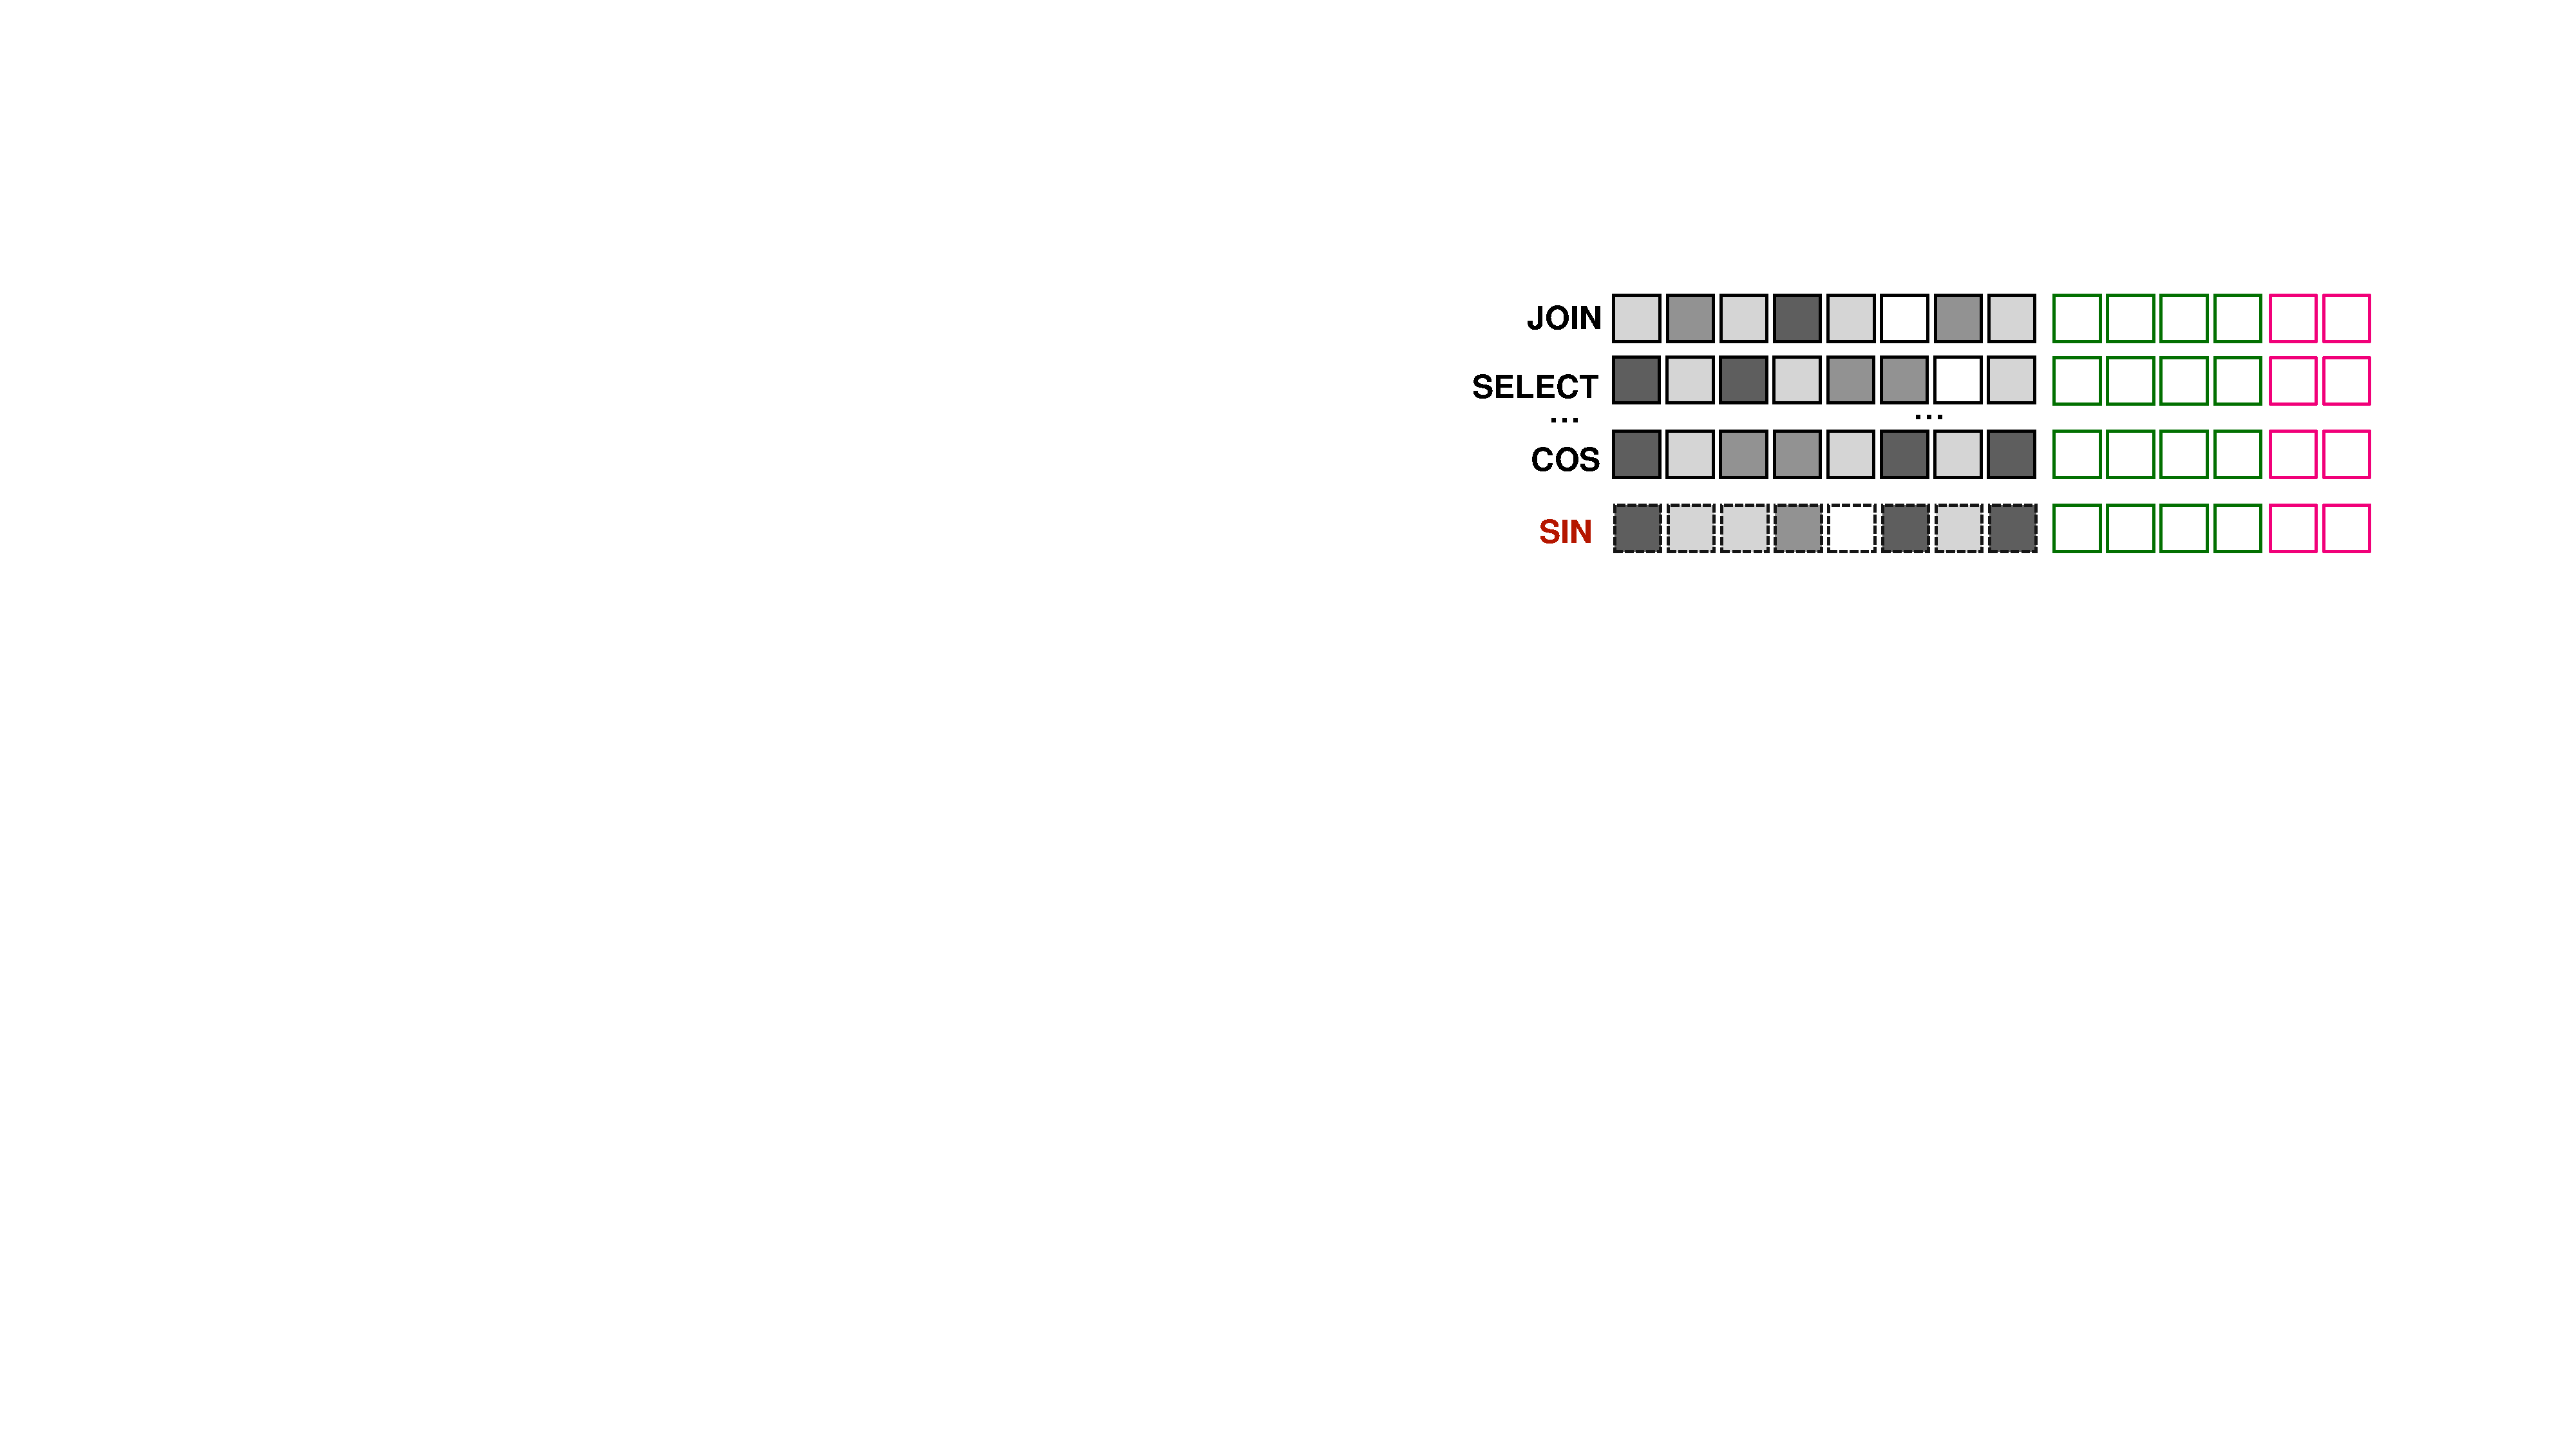
\includegraphics[width=0.45\linewidth]{figures/feature-vector-embedding.pdf}
  } 
  \caption{Feature Vector Comparison}
  \label{fig:feature-vector}
\end{figure}

However, this encoding has two prominent limitations that are especially obvious in CLIC:

1) Low computational: 
The dimension of the one-hot encoding is equal to the category amounts and the vector has only one non-zero element.
Therefore, as the number of categories grow up, the one-hot encoding usually resulting in a high-dimensional and sparse vector. 
Generally speaking, this makes it less computational since the majority of neural network toolkits do not play well with very high-dimensional, sparse vectors [Neural Network Methods in Natural Language Processing, 2017]. 
Since a cross-platform framework like CLIC usually need to train a cost model but face the insufficient training data problem, 
this limitation becomes more crucial to them.

2) Imcompatible to a new operator integration: 
In particular, as a new operator been integrated, the dimension of the one-hot vector will grow in the same time. 
Figure \ref{fig:feature-vector-onehot} examplified this situation. 
When the new \textit{SIN} operator (the red operator) being inserted, all the vectors' dimensions are grown by one (represented by dash line).
The consequnce is that the pre-trained model, GCN for example, needs to be retrained because the higher dimension conflicts with the model's input requirement.
This problem does not exist in most scenarios, because the dimensions of the input data are usually predefined and will not grow.
However, as we have narrated in Section 2, a cross-platform system experiences fast evolutions, such as enriching the operator library.
Under this circumstance, the dimension of the one-hot vector will vary frequently, which further lead to the frequent model retraining.


In order to overcome the above two limitations, we propose a novel feature extraction method called operator embedding.
% 为了克服以上两个问题,我们提出了新的使用运算符嵌入(operator embedding)向量化运算符的方式。

\textbf{Operator Embedding}
In mathmatic, an embedding is a function $f X -> Y$ that maps a data point X in one space to point Y in another space[wiki]. 
This is the most important preprocessing technique in natural language processing (NLP), where the word embedding is a term used for the representation of words for text analysis. 
It is typically in the form of a real-valued vector that encodes the meaning of the word such that the words that are closer (cosine distance) in the vector space are expected to be similar in meaning [wiki]. 
For promotion, there also are image embedding, video embedding. 
A representative algorithm for generating word embedding is the CBOW[], whose idea is that words appearing in the same sentence have higher relevance. 
The way CBOW works, in a nutshell, is that it tends to maximize the joint probability of a word and its context words in a sentence. 
Generating the word embedding using CBOW requires a large corpus containing enough sentences as the training dateset to learn the word relationships.

Back to CLIC, we assume that operators also have semantical meanings and are relevant to the others in the same logical plan.
The semantical meanings, for example, include operator's computing paradigm, \#input/output, etc.
Based on these assumptions, we design the operator embedding.

As illustrated in Figure \ref{fig:feature-vector-embedding}, 
the operator embedding is a real-valued continuous vector whose dimension is fixed (hyper parameter) and usually rather smaller than that of the one-hot encoding.
It has two key characteristics that can overcome the above one-hot encoding's limitations:
1) Low-dimensional and Dense. 
Compare to one-hot encoding's high-dimensional 0-1 vector, 
the operator embedding is encoded with real-world meanings and therefore only a low-dimensional vector is required to represent an operator.
This makes it more computational for the following models, and in the meantime, saves a lot of training data.

2) Compatible to the operator evolution. The embedding's dimensions will not grow with the integration of new operators. 
As we can see from Figure \ref{fig:feature-vector-embedding}, the newly integrated \textit{SIN} operator has consistent dimension with the others.
The model that takes it as input data does not need to be retrained anymore. 
This largely supports the fast evolution of CLIC.

To generate the operator embedding, we share the same ideas in the word embedding that
1) allowing semantically similar operators to have closer (cosine) distance, 
and 2) maximizing the joint probability of an operator and its neighbour operators in a logical plan.
Therefore, we can still adopt the CBOW algorithm.
We consider the topological ordered logical plan as the "sentence", where each operator is a "word" and its neighbors are the "context words". 
The corpus, i.e. logical plan dataset, are retreived from our synthesized dataset which will be discussed later in Section xx.
Using this corpus as dataset, we finally have the trained operator embeddings visualized in Figure \ref{fig:emb_visual}.
We reduce the dimension to the top-2 dimensions with the highest eigenvalue for the sake of visualization.
The observation is that the operator \textit{sin} is closer to \textit{tan} and far from \textit{union}.
This can be explained semantically as that \textit{sin} and \textit{tan} belong to the same computing paradigm and have the same \#inputs/outputs.
Although the meanings of the embedding are more complex than just paradigm and parameter amounts, 
for CLIC, 
we can simply assume that the operator embedding has successfully portrays the operator.
The power of the embedding will further be revealed when utilizing to train the GCN model, which we will disscuss in Chapter xx.

\begin{figure}[tbh]
  \centering
  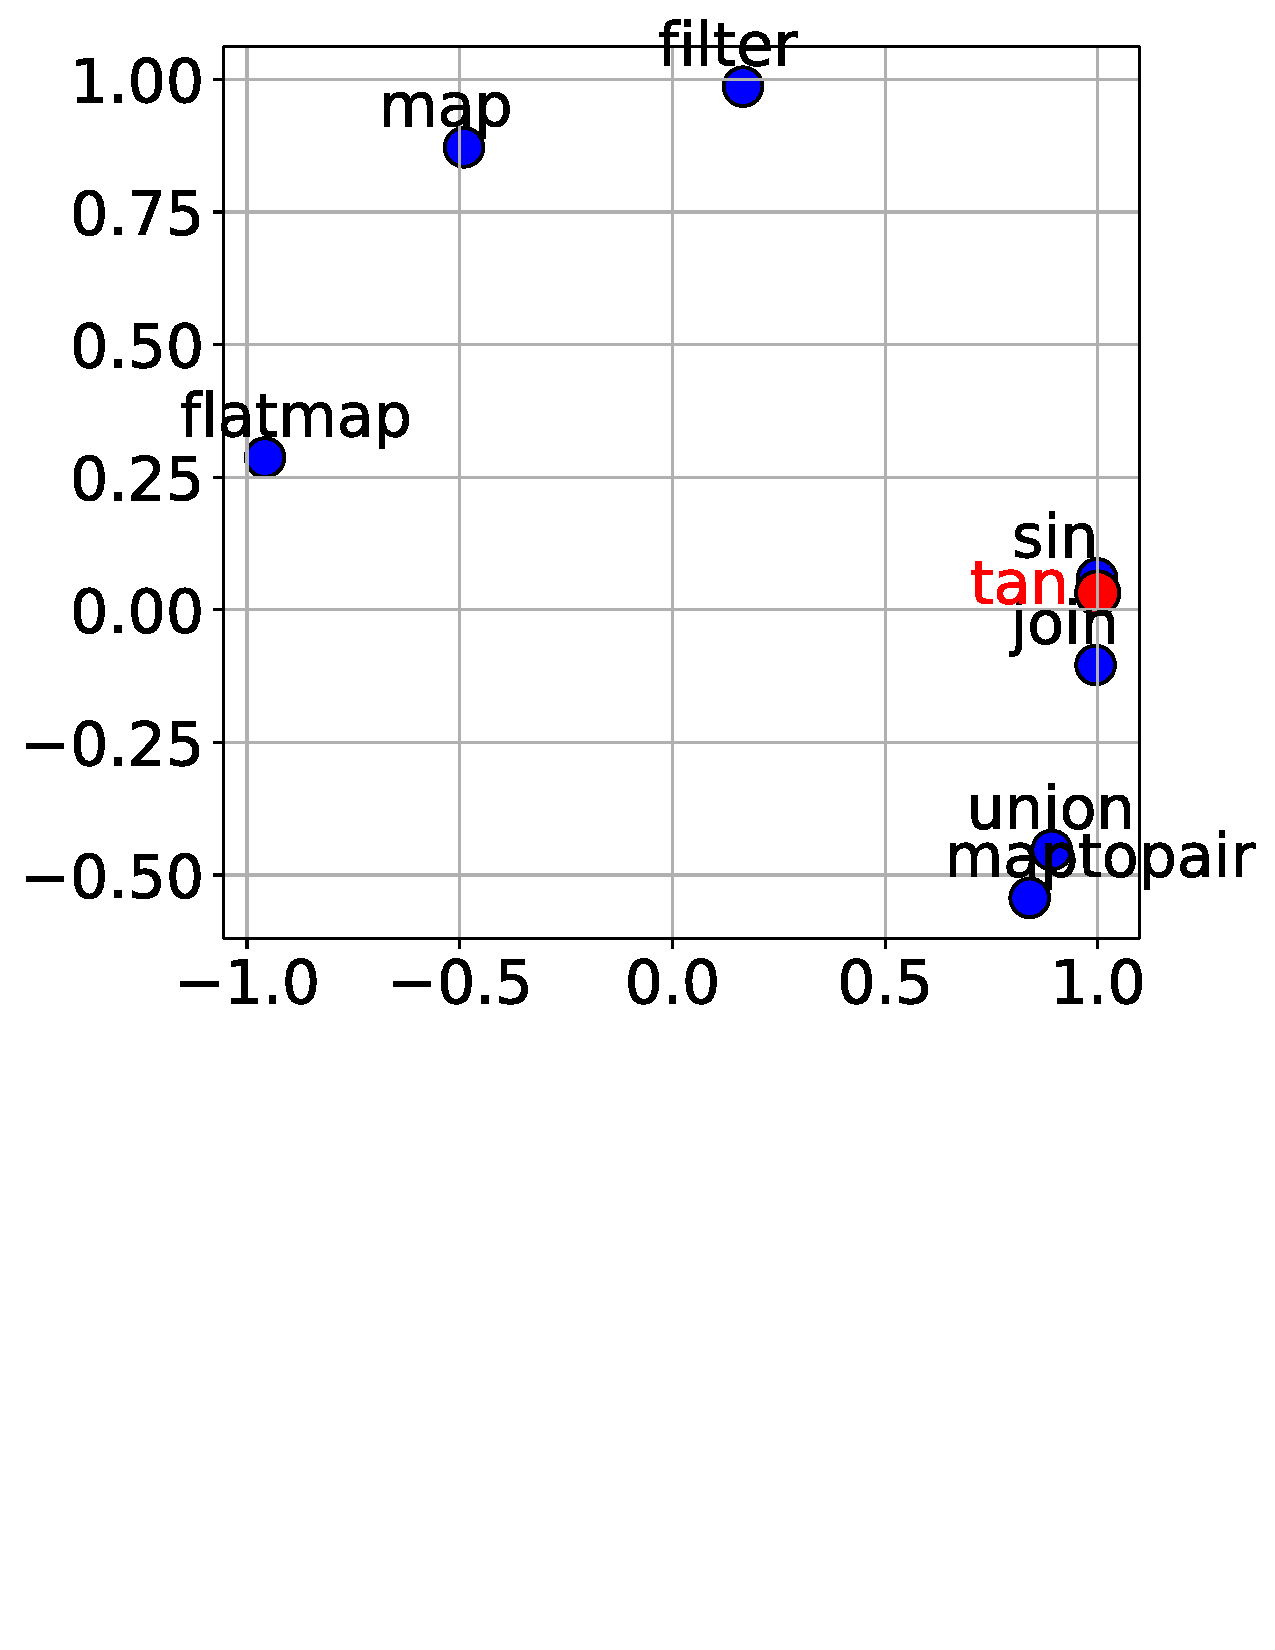
\includegraphics[width=0.6\linewidth]{figures/embedding_visual.pdf}
  \caption{Visualization of the trained operator embedding}
  \label{fig:emb_visual}
\end{figure}

One thing we want emphasize is that,  
since the operator used as the input of embedding is only logical,
one can generating an operator's embedding whether it is actually implemented by a framework, say CLIC, or not, 
as long as the corpus they offered contains the operator.
In another word, the operator embedding technique is a general encoding method that is independent to any computing frameworks.
What this means to CLIC is that, we can construct a rich operator embedding set as the "dictionary" before we actually implement them.
After that, every time we integrate a new operator, we look up to the dictionary for its embedding. There are two scenario for getting the embedding:
1) The operator is new to CLIC but not the dictionary. In this case, we retreive its embedding directly from the dictionary.

2) The operator is "Out-Of-Vocabulary (OOV)". In this case, we need to first synthesize some new logical plans that contain this operator according to its attributes (paradigm, \#input/output, etc.), and then re-generating all of the embeddings.


\subsubsection{Hardware}
Hardware resources such as network bandwidth, GPU memory, SSD/HDD, etc. are also important factors affecting platform classification. 
For example, the selection of two different communication model used in ML frameworks, i.e. the parameter server model and the all-reduce model, are effected by the bandwidth and the GPU. 
In general, the parameter server works better if you have a large number of unreliable and not so powerful machine;
All-reduce works better if you have a small amount of fast devices(variance of step time between each device is small) run in a controlled environment with strong connected links. 
The benchmark result in [ML platform Benchmark] and the experiments in Section 2 also support to this. 
Therefore, we also encode the hardware parameters into the feature vector, as shown in the green segment in Figure \ref{fig:feature-vector}. 
Those features are the same for all operators in a logical plan. 

% The Figure xx.3 is the classification result of the same plan with the operator platforms are changed from Tensorflow to PyTorch. 
% The reason behind it may be that the network card has been upgraded from 9GBS to 200GBS and the communication model of Tensorflow is set to the parameter server by default, and vice versa for PyTorch. 

\subsubsection{Workload}
% 数据分布和 selectivity
% 还没想好怎么写



Put it all together, the final feature vector consists with the operator embedding, hardware, and workload.
We adopt a 8-dimension embedding, and therefore get the final 8 + 4 + 2 = 14-dimension feature vector, as shown in Figure \ref{fig:feature-vector-embedding}.
The gray, green, and pink segments respectively represent the above three factors.
Next, we are going to introduce how GCN utilizes this feature vector to do node classification.

\subsection{GCN Intuition}

Graph Convolutional Network is a convolutional neural network that can be directly applied to graphs. 
It applys the convolution kernel to learn the first-order spectral feature, which are followed by activation functions to learn graph representations[42]. 
The convolution kernel learns the spectral feature by inspecting neighboring nodes in turn. 
Below we introduce the logical plan's node classification process using GCN, which is shown in Figure \ref{fig:gcn}.

\begin{figure}
  \centering
  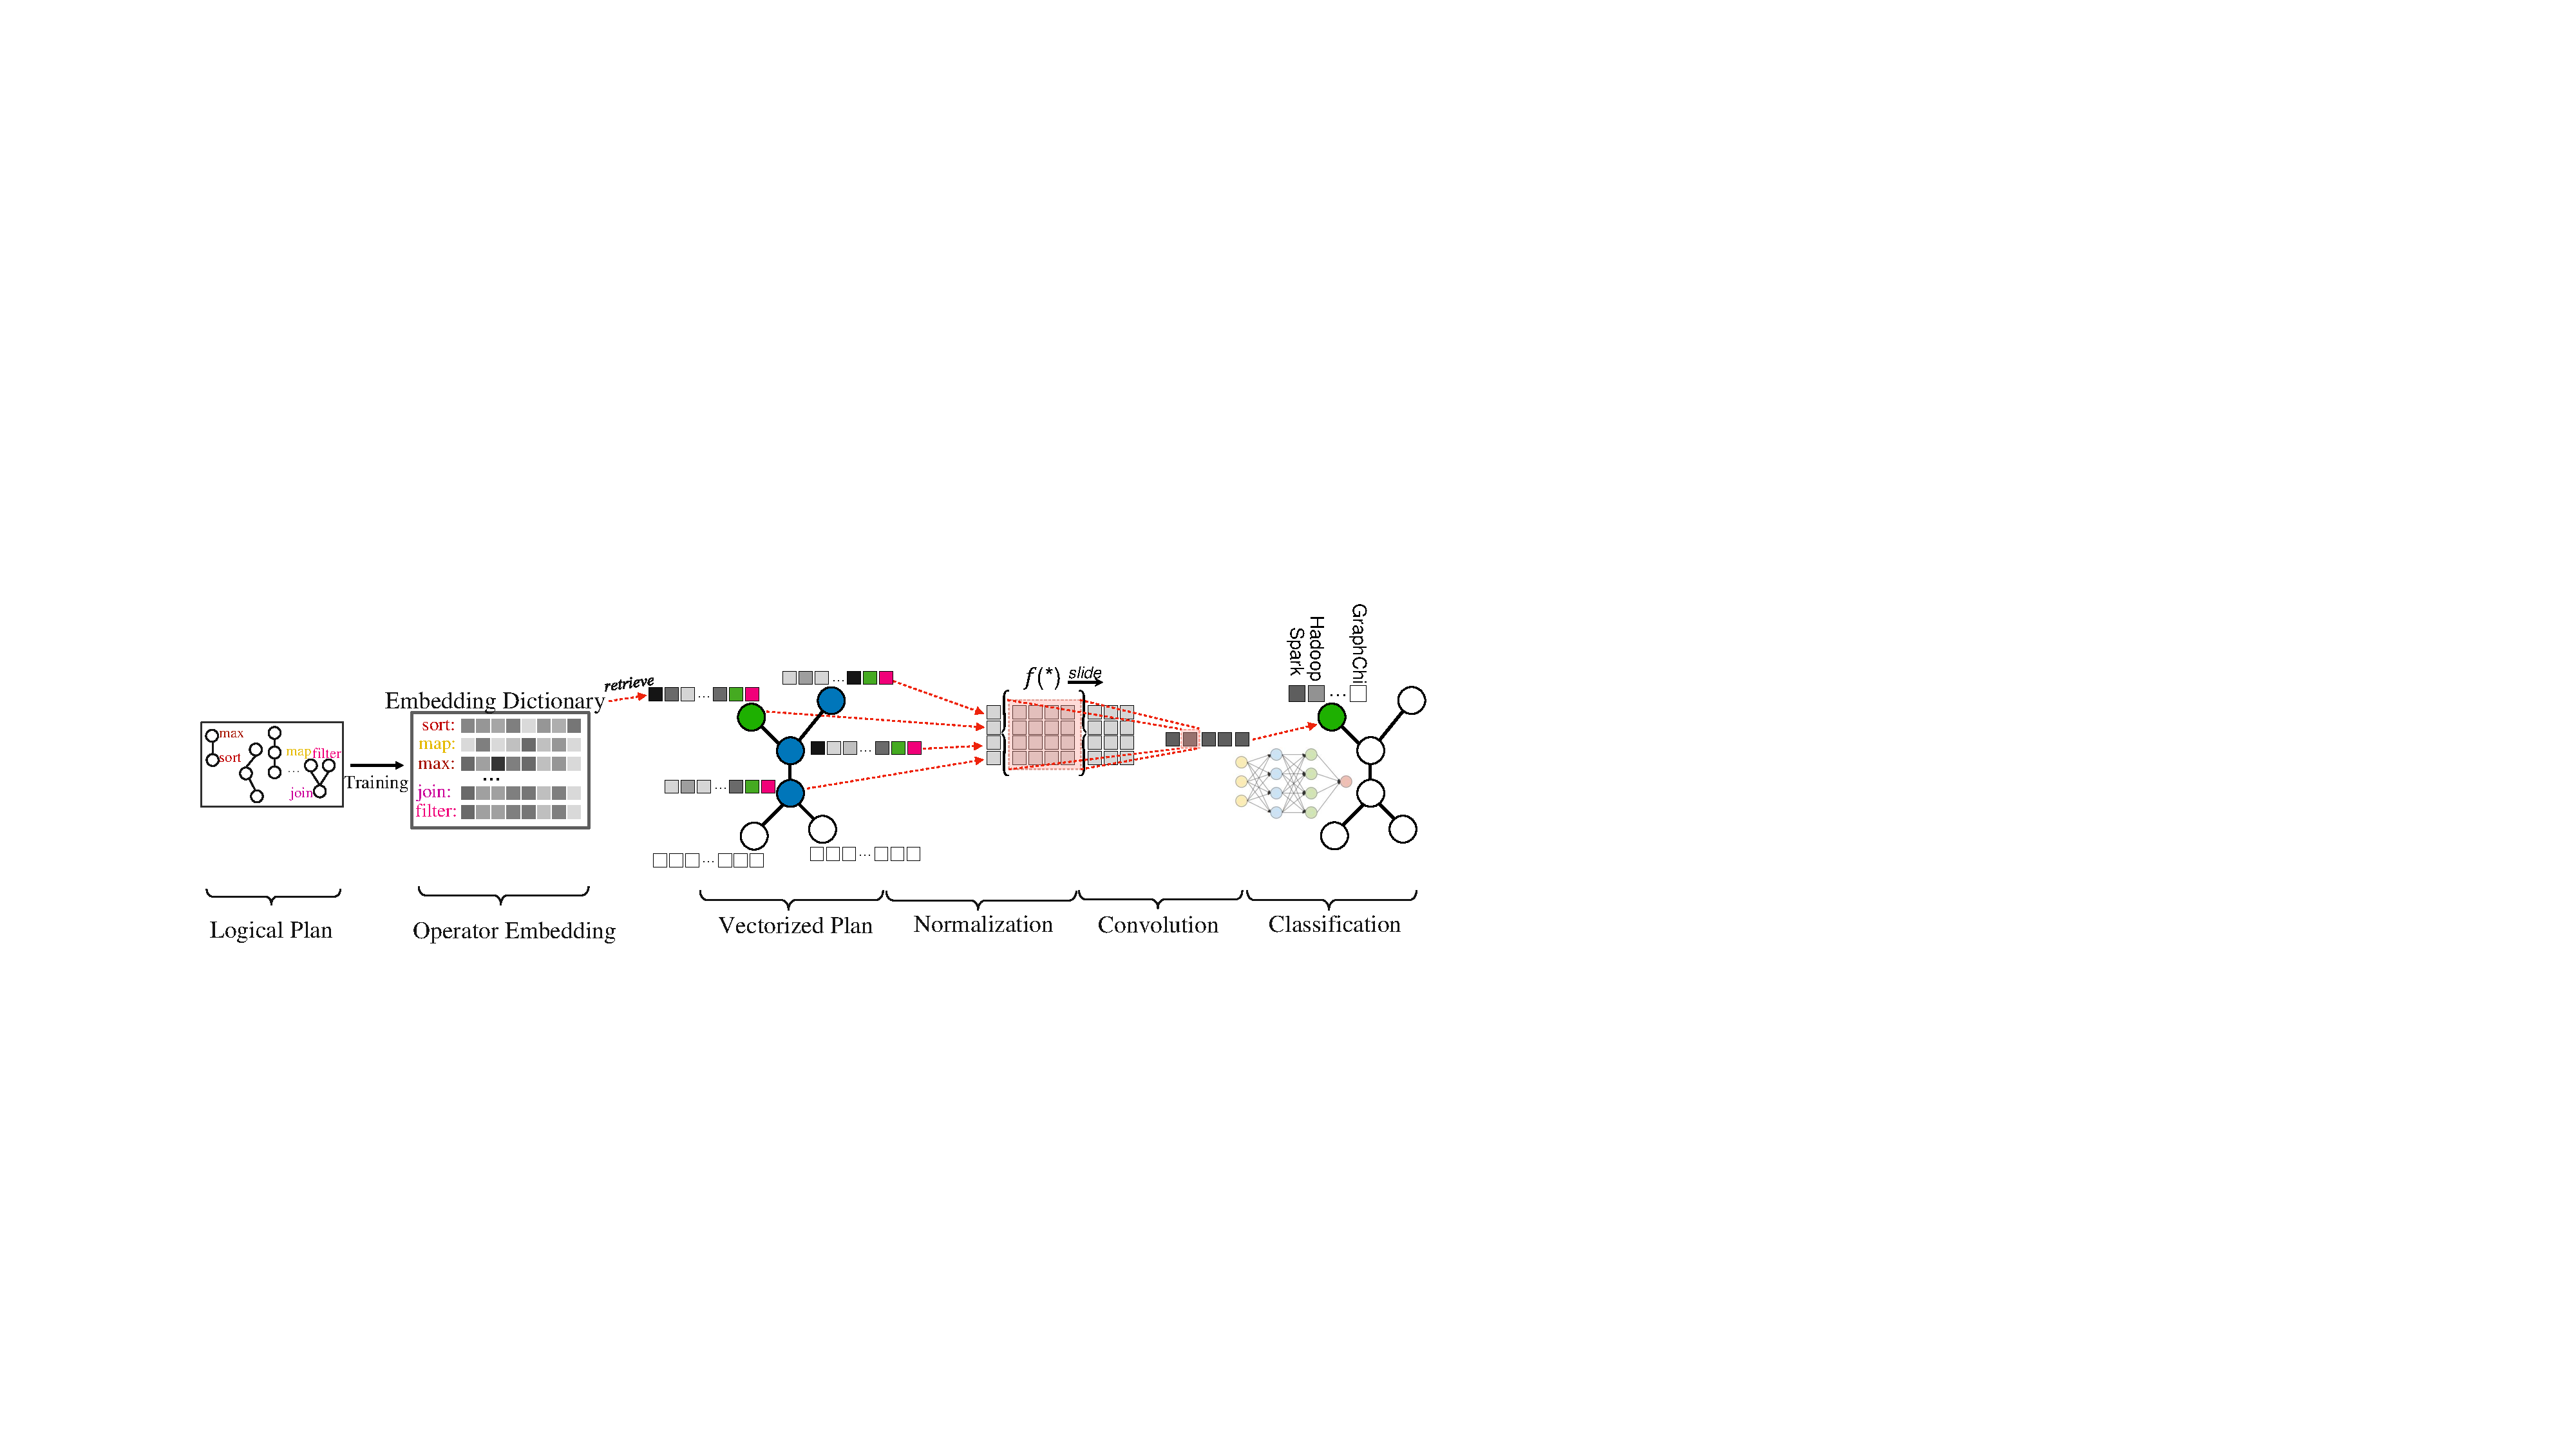
\includegraphics[width=\linewidth]{figures/GCN-new.pdf}
  \caption{Selecting platforms with GCN}
  \label{fig:gcn}
\end{figure}

The input of GCN is a graph with nodes are represented as vectors $\vec{V}$. \
The vector $\vec{V}$, as we have just disscussed, consists with three segments: operator embedding (gray), hardware (green), and workload (pink).
The hardware and workload are computed runtime by CLIC and are the same to all nodes, 
while the operator embedding is retreived respectively from the pre-generated embedding dictionary.
In order to learn the relationship between the current operator (green node) and its neighbors (blue nodes), 
the input topology needs to experience alignment and convolution steps.
The alignment step aligns the irregular topology to the matrix. 
This is done by selecting the current operator and its K-1 neighbors to form the matrix of size $K * |V|$. 
Then during convolution step, the kernel function \footnote{The kernel function takes as input a matrix, 
then dot products it with another pre-defined matrix, 
and finally aggregates the resulting matrix to a scalar.} slides $f(x)$ across the matrix.
Since each time the kernel function outputs a scalar, the result of this step is a vector that represents the aggregation of the operator and its neighbors. 
In our classification case, the aggregation vector is utilized for classifing the operator.
The output of the classification step is the probability distribution of all available platforms, \
of which, the one with highest probability is selected as the resulting label.
This probability distribution is computed by what we really need to train, the neural network.


\subsection{Training GCN}
The training data is a logical plan, among which each operator has an input vector along with a label.  
Since the effectiveness of the model depends on the quality of the dataset. 
a large number of logical plans are required first. 
In order to get the labels of each plan, we also need to actually run all of its possible physical plans with different workloads and infrastructures, and choose the one with the least execution time. 
But this confronting two chanllenges: 
i) there lacks sufficient real-world logical plans [] and 
ii) it's impossible to run all the possible physical plans since it is an exponential search space. 

For the former problem, we used the synthesis way to generate the traning data. 
We construct a state machine for each computing paradigm respectively to represent its programming model, and synthesize the actual logical plans using the markov chain. 

For the latter problem, we first prune the search space using the technique in []. 
And for the last physical plan, we specified the data source and several workloads, and run them to get the labels, then we populate the data by interpolation []. 
At last, we repeate the above steps on variational infrastructures.

We train the GCN model using the above synthesized dataset and Figure xx shows the model accuracy on the collected real-world test set. 
It can be seen that, the model acquires pretty good result on the single computing paradigm. 
However, when dealing with the large graph, especially the hybrid graph, the accuracy drops to nearly 50\%, which is unacceptable.

One of the main problem is the one-hot encoding. 
This encoding method always results in a high-dimensional and sparse vector. 
Generally speaking, this makes it less computational since the majority of neural network toolkits do not play well with very high-dimensional, sparse vectors [Neural Network Methods in Natural Language Processing, 2017]. 
The less computational problem is crucial to such a framework since it already faces the insufficiant data problem. 

Another side-effects of the one-hot encoding is that it is imcompatible to a newly integrated operator, which goes against to our high extensible character. 
In particular, the one-hot encoding needs to increase the dimension of all operator vectors whenver a new one is inserted. 
Figure xx examplified this situation where as the new Flatmap operator (red one) being inserted, all the vectors' dimension are grown. 
Thus the previous model needs to be retrained otherwise the new vector becomes an invalid input due to its higher dimension. 
Even if reserving some empty dimension to stablize the input, the model still cannot properly classify the new operator because the new dimension is orthogonal to the other dimension and the model lacks knowledge about this new dimensions.

In order to overcome the above two problems, we turned our attention to represent the operator using the embedding.


% \begin{figure}
%     \subfigure[One-Hot Encoding]{
%         \label{fig:one-hot}
%         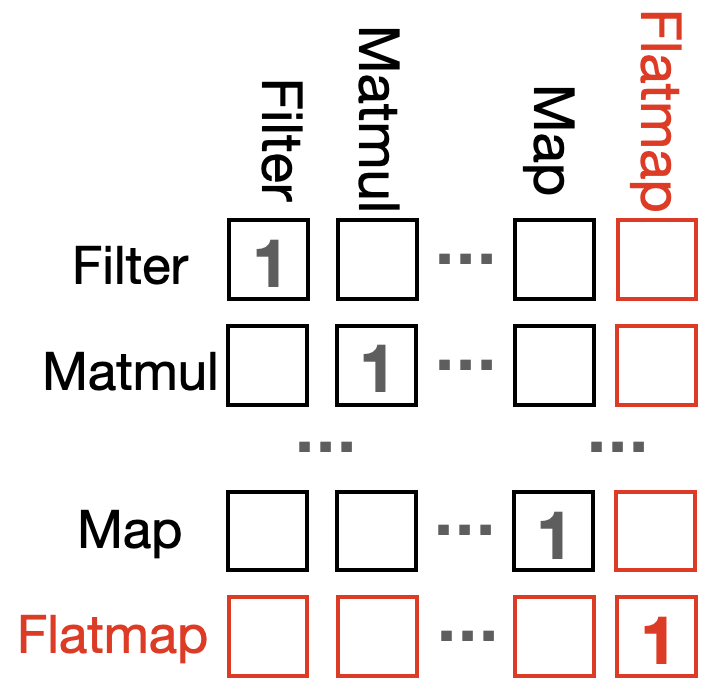
\includegraphics[width=0.3\linewidth]{figures/one-hot.png}
%     } 
%     \subfigure[Operator Embedding]{
%         \label{fig:embedding}
%         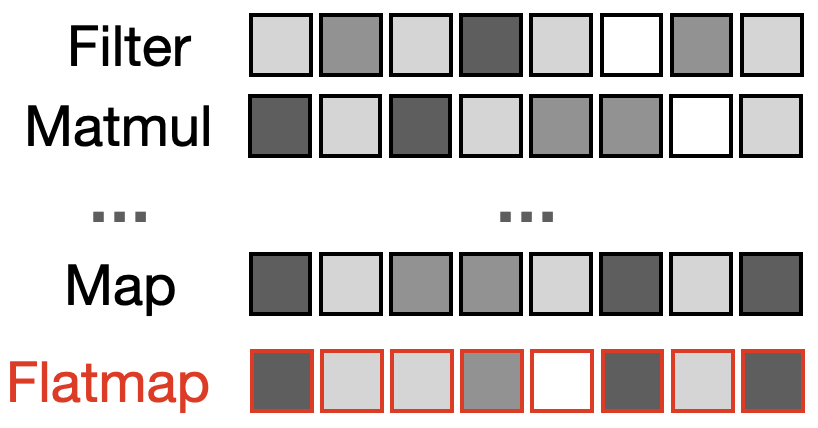
\includegraphics[width=0.3\linewidth]{figures/embedding.png}
%     } 
%     \caption{Vectoization Method}
%     \label{fig:encoding}
% \end{figure}


% \subsection{Data Generation}
% \textbf{Generating Operator Embedding}
% In word embedding, because the words in a sentence have certain correlation with its context words, 
% the cost function of training Word Embedding is to maximum the joint probability of the word and its context words. 
% Similarly, we can also reasonably assume that the operators that appear in a same logical plan have certain correlation and use the same cost function. 
% We take the topological-ordered logical plan as the sentence and the logical operators inside are words, 
% then use the same model to train the operator embedding. The results are shown in Figure xx. 
% For the sake of visualization, we just show the top-2 dimensions with the highest eigenvalue. 
% One observation is that operators that are the same computing paradigm and have the same number of inputs and outputs tend to have small cosine distance. 
% What's more, the newly inserted Flatmap operator is also mapped closer to the Map operator instead of the Matmul operator which is probably due to the same reason.

% % TODO: 图之后再调整
% \begin{figure}
%     \subfigure[Operator Embedding]{
%         \label{fig:opt_ebd}
%         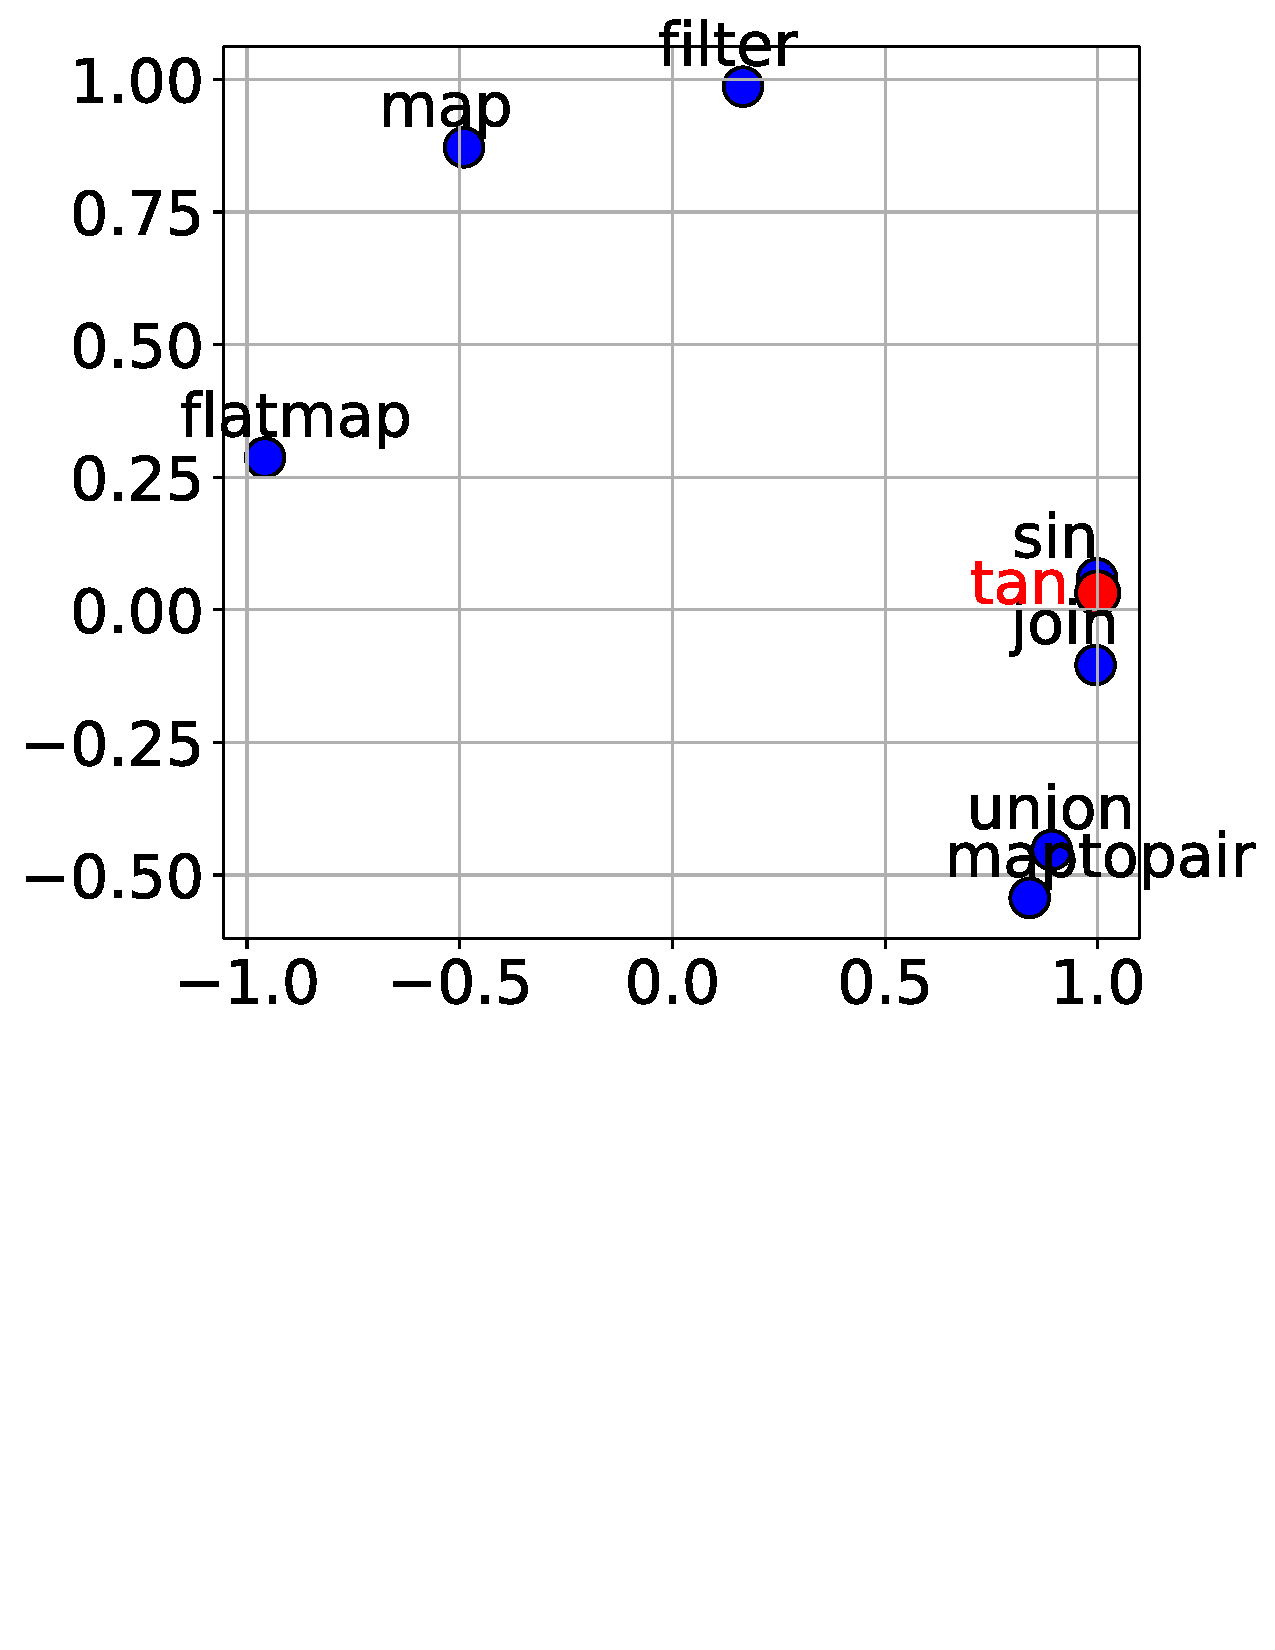
\includegraphics[width=0.4\linewidth]{figures/embedding_visual.pdf}
%     } 
%     \subfigure[Platform Embedding]{
%         \label{fig:embedding}
%         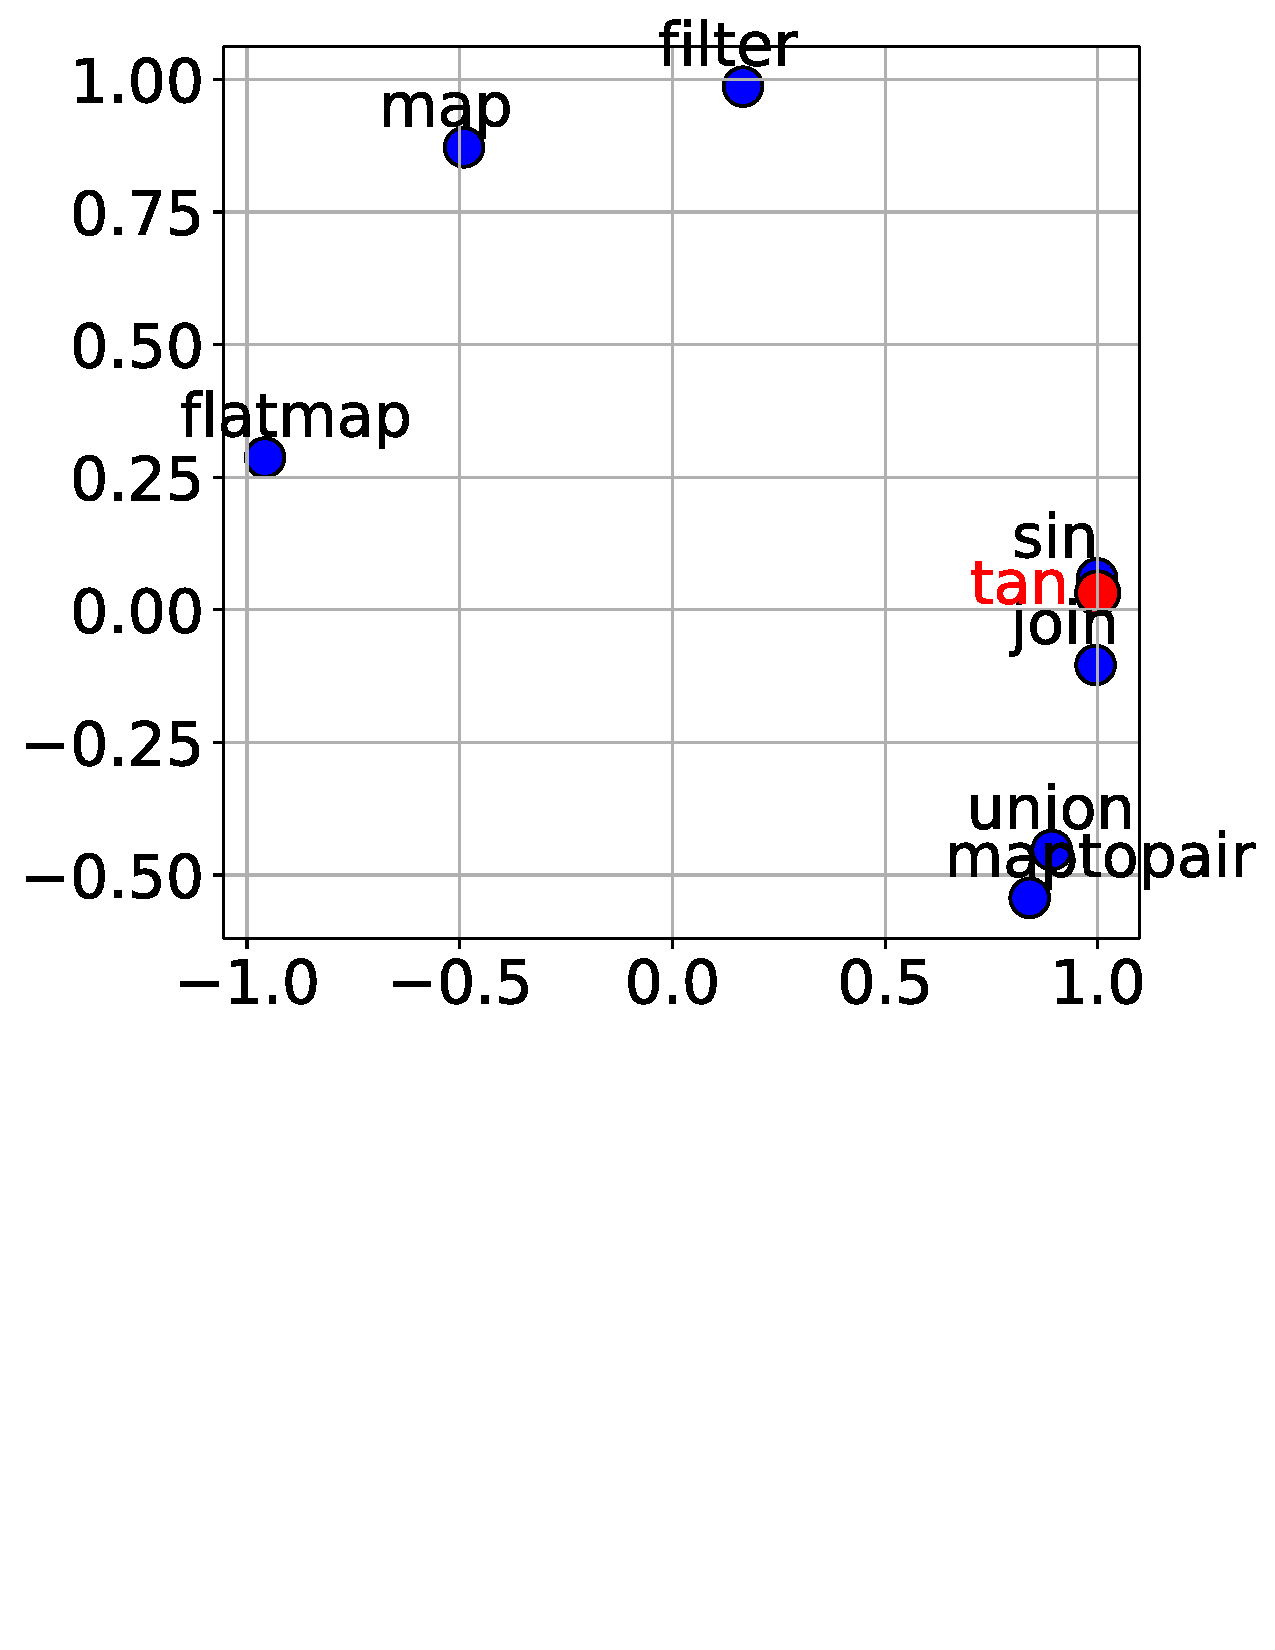
\includegraphics[width=0.4\linewidth]{figures/embedding_visual.pdf}
%     } 
%     \caption{Embedding Visualization}
%     \label{fig:embedding_panel}
% \end{figure}

% It's important to emphasize that the operator embedding technique is not bound with CLIC but a general feature extraction method. 
% One can generate an operator embedding whether the operator is supported by CLIC or not as long as there are logical plans that contain this operator.

% As we have mentioned that the operator embedding is compatible for the newly integrated operator. 
% There're two cases when integrating a new operator:
% \begin{itemize}
%     \item [1)]
%     The operator is new to CLIC but not the model, therefore its embedding can be retreived in CLIC directly from the model.
%     \item [2)]
%     The operator is also new to the model, i.e. the "OOV" (out of vocabulary) problem. 
%     In this case, the model needs some new training data to recognize it. 
%     Therefore, we synthesize some new logical plan that contains the operator according to operator's attributes and then incrementally updates the model to generate the embedding.
% \end{itemize}

% Apart from the above operator embedding, 
% we also design and generate the embedding for each physical computing platform. 
% The mathmatical meaning and generation method goes the same. 
% We don't further explain due to limits of space.


% \textbf{Generating Training Data}
% The effectiveness of the GCN strongly depends on the training data. 
% In our case, a large amount of disparate logical plans (data points) together with the best physical platform (labels) of each logical operator in it is required. 
% The logical operator's feature vector is composed of two parts: operator embedding and the global hardware resources. 
% % 1. 举例子说明为什么考虑带宽
% % 2. 把向量图画出来
% % 3. 把这段提前
% The latter is the same for the operators in the same logical plan, including infrastructure's CPU frequency, main memory, GPU memory, network bandwidth, etc. 
% However, there is currently a lack of the Workflow dataset for cross-platform computation, so we borrow the TDGen [] to synthesized datasets separately for each computation mode and on different infrastructures.